\documentclass[a4paper]{article}

\input ../header
\usepackage{minted}
\usepackage[np]{numprint}
\usepackage{lscape}
\usepackage{afterpage}
\usepackage{hyperref}

\setlength{\multicolsep}{2pt}

% Commandes pour cacher/révéler du texte facilement à l'aide d'un booléen
\usepackage{xstring}
\usepackage{ifthen}

\newboolean{reveal}
\setboolean{reveal}{false}

\newlength{\stextwidth} % une nouvelle longueur

\newcommand\x{6}

\newcommand{\guess}[1]{\ifthenelse{\boolean{reveal}}{{\color{red}#1}}{\settowidth{\stextwidth}{#1}\makebox[\stextwidth]{\dotfill}}}

\newcommand{\guessmath}[1]{\ifthenelse{\boolean{reveal}}{\textcolor{red}{#1}}{\settowidth{\stextwidth}{$#1$}\makebox[1.9\stextwidth]{\dotfill}}}

\newcommand{\guessmathbin}[1]{\ifthenelse{\boolean{reveal}}{\mathbin{\color{red}#1}}{\settowidth{\stextwidth}{$#1$}\makebox[2\stextwidth]{\dotfill}}}

\begin{document}

\title{Le Web -- Activité 3}

\pagestyle{empty}

\date{}
\author{}

\maketitle{}

\thispagestyle{empty}
\noindent\textbf{Activité 3}\hfill{}\textbf{Ma première page Web}
\smallskip
\hrule
\medskip

Les pages Web sont écrites à l'aide de langages qui permettent d'afficher leurs contenus. Cette activité est une activité d'introduction aux langages HTMl et CSS.

\begin{enumerate}
  \item Que signifient les acronymes HTML et CSS ?\rep{6}
  \item Compléter le texte suivant :
    
    \medskip

    \og{}Le $\hdots\hdots\hdots\hdots$ est un langage qui permet de placer les éléments d'une page Web (textes, liens, sons, photos etc) sur celle-ci et de l'afficher dans un $\hdots\hdots\hdots\hdots\hdots\hdots$\fg{}

    \medskip

    \og{}Le $\hdots\hdots\hdots\hdots$ est un langage qui permet de gérer la $\hdots\hdots\hdots\hdots\hdots\hdots$ d'une page en définissant les propriétés qui devront être appliquées pour chaque élément de la page.\fg{}
  \item Voici à quoi ressemble un fichier HTML basique :
    \begin{center}
      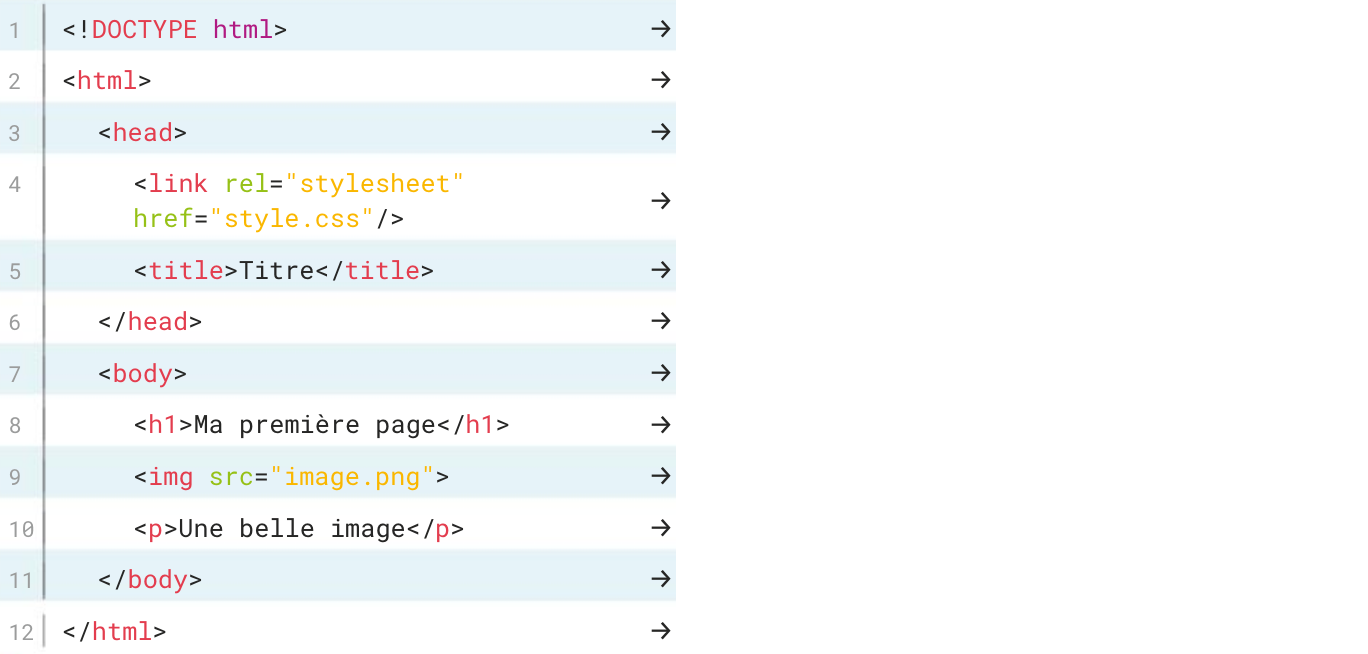
\includegraphics[width=16cm]{page_HTML_de_base.png} 
    \end{center}
    Expliquer le rôle de chaque ligne de ce fichier.
  \item 
    \begin{enumerate}
      \item Saisir le code HTML précédent dans un \textbf{éditeur de code} : sur les postes du lycée, utiliser par exemple Notepad++. Avec un iPad du lycée, utiliser Coda.
      \item Sauvegarder le fichier sous le nom \verb|index.html| puis l'ouvrir dans un navigateur. Que constate-t-on ?\rep{6}
	\pagebreak
      \item Le fichier \verb|style.css| auquel fait référence la ligne 4 du fichier HTML n'existe pas encore. Voici son contenu :
	\begin{center}
	  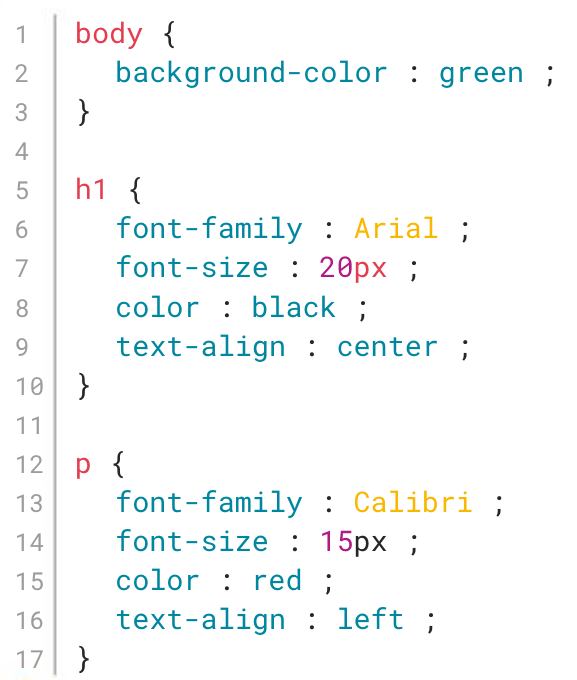
\includegraphics[width=7cm]{style.css.png}	
	\end{center}
    \end{enumerate}
    Créer le fichier \verb|style.css|, le sauvegarder dans le même répertoire que le fichier \verb|index.html|.
  \item Rafraîchir la page \verb|index.html| dans votre navigateur. Que constate-t-on ?\rep{4}
  \item Expliquer alors le rôle de chaque ligne du fichier \verb|style.css|.
  \item Comment définir des listes ordonnées en HTML ? Donner un exemple.\rep{6}
  \item Comment définir des listes non ordonnées ? Donner un exemple.\rep{6}
  \item Comment créer un lien hypertexte ? Donner un exemple.\rep{6}
\end{enumerate}

\bigskip

\textbf{Travail à réaliser et à déposer sur Moodle}

\medskip

Réaliser une page HTML sur le sujet de votre choix. La page comportera tous les éléments vus dans cette activité.

\end{document}
